\documentclass[../report.tex]{subfiles}
\begin{document}

\graphicspath{{img/}{../img/}}

\section{Activity Breakdown}

\label{sec:Activity Breakdown}

Et activity breakdown diagram laves ved at se p� hvilke ting der skal udf�res for at et projekt bliver f�rdigt. Man inddeler alts� projektet i aktiviteter og n�r alle aktiviteter er udf�rt er hele projektet udf�rt. Hver aktivitet kan s� inddeles i mindre aktiviteter. Ligesom et product breakdown diagram danner disse aktiviteter et hierarki hvor den �verste aktivitet vil v�re at udf�re hele projektet og de nederste aktiviteter vil v�re detaljerede aktiviteter som er mere overskuelige at arbejde med. \\

\noindent
Ved at lave et activity breakdown diagram f�r man brudt den aktivitet det er at lave et helt projekt ned i nogle mindre aktiviteter. Det g�r det blandt andet nemmere at estimere et projekt fordi det er nemmere at estimere hvor lang tid det tager at lave en lille del (en database fx) end det er at estimere hvor lang tid et helt projekt tager. Det giver ogs� mulighed for at se p� hvordan aktiviteterne afh�nger af hinanden s� man kan prioritere hvad der skal laves f�rst. \\

\noindent
I target-projektet blev der lavet et activity breakdown diagram som ikke bryder aktiviteterne i projektet helt ned i atomiske aktiviteter. Aktiviteterne er blevet holdt p� et nogenlunde abstrakt niveau fordi der blev arbejdet med Scrum som procesmodel i target-projektet. Det var derfor ikke n�dvendigt at bryde alle aktiviteter ned i atomiske dele i starten af projektet. Den nedbrydning fandt sted l�bende n�r der blev holdt m�der i forbindelse med sprintplanl�gning. Et eksempel p� en s�dan nedbrydning kan ses p� figur (FIGUR REF HER). Hvis man derimod havde brugt vandfaldsmodellen som procesmodel, havde det v�ret n�dvendigt at nedbryde alle aktiviteter s� meget s� muligt fra starten af projektet, for at kunne estimere bedst muligt. \\

\noindent
Da det activity breakdown diagram der blev lavet i target-projektet, ikke er brudt helt ned i atomiske aktiviteter, blev det ikke brugt til en dataljeret estimering af projektet, men mere til at planl�gge hvilke aktiviteter der skulle udf�res f�rst. Der blev ogs� lavet et Gantt-chart, som ud over at beskrive den r�kkef�lge aktiviteterne skulle udf�res i ogs� indeholdt en l�s tidsplan for projektet baseret p� activity breakdown diagrammet.

\newgeometry{left=5cm,bottom=1.4cm}
\begin{landscape}

\subsection{Activity Breakdown Diagram}

\begin{figure}[H]

\label{fig:Activity Breakdown Diagram}
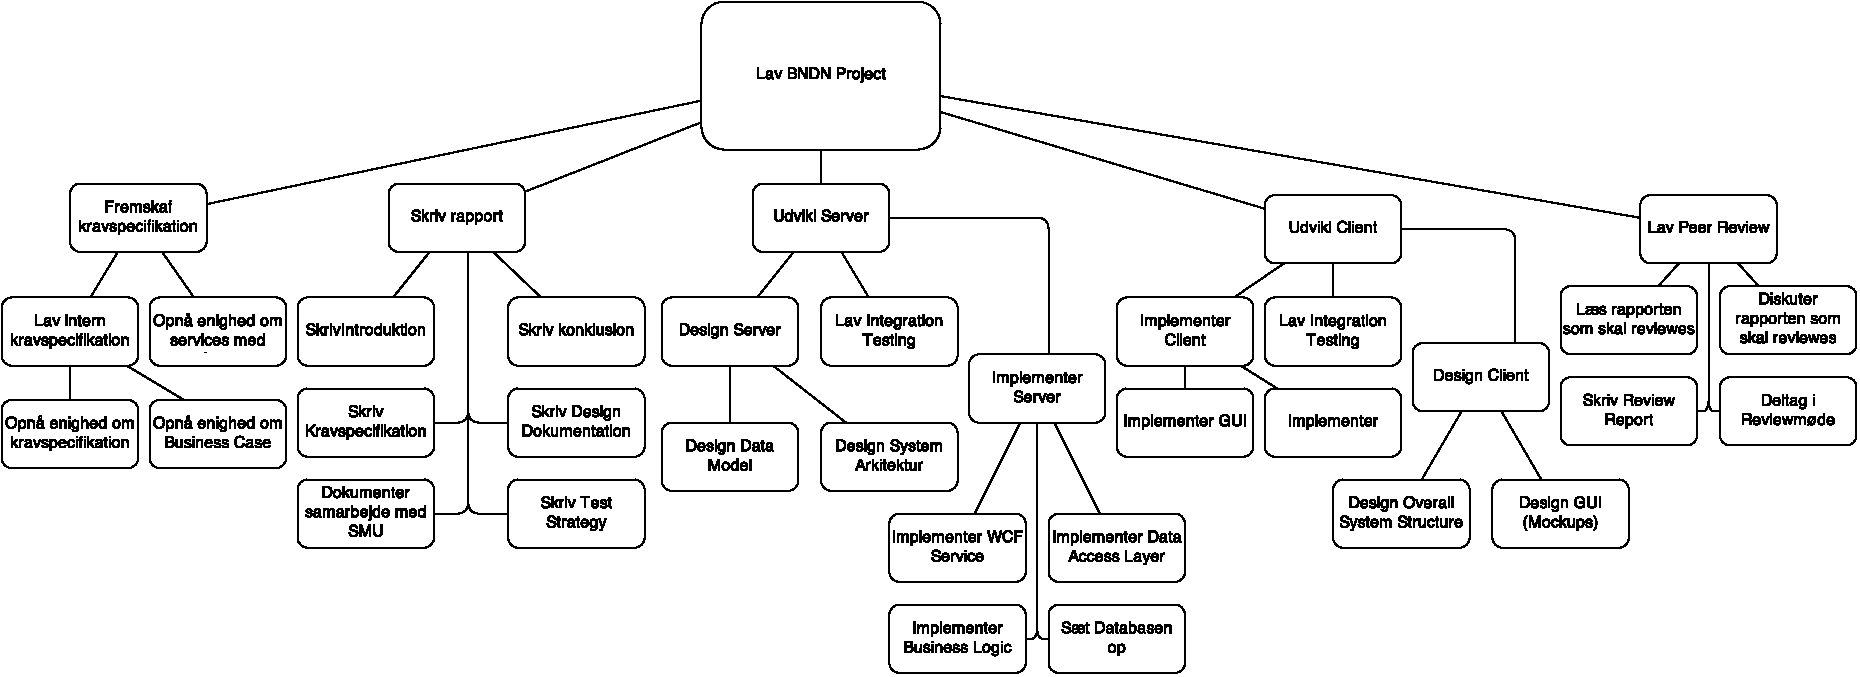
\includegraphics[ scale=0.84]{ActivityBreakdownDiagram.pdf}
\caption{Activity Breakdown Diagram}

\end{figure}

\end{landscape}

\end{document}